\section{The Blaze Library}
\label{sec:blaze}
The Blaze library offers three sets of APIs: 1) a high-performance MapReduce function, 2) distributed data containers, and 3) parallel computing utility functions.
These APIs are built based on the Blaze parallel computing kernel, which provides common low-level parallel computing primitives.

% Blaze also offers several utility functions for parallel programming, including thread-safe random number generators, a parallel file loader, and converters between C++ standard library containers and Blaze distributed data containers.


\begin{figure}
  \begin{center}
  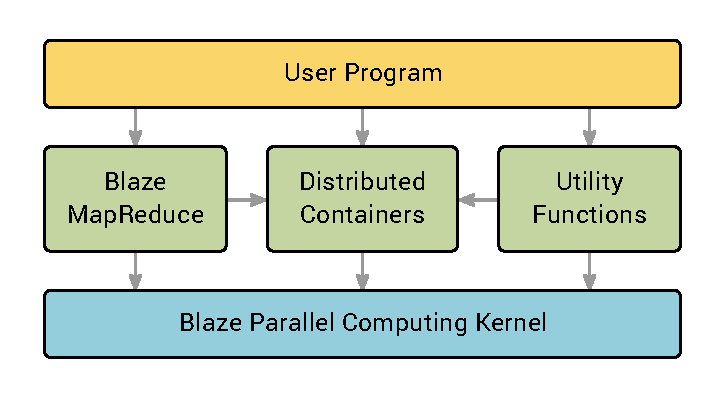
\includegraphics[width=\linewidth]{arch0.eps}
  \end{center}
  \vspace{-0.2cm}
  \caption{Blaze Architecture.
%   Blaze exposes three sets of APIs: the high performance Blaze MapReduce function, distributed data containers, and a few utility functions.
%   The Blaze parallel computing kernel provides low-level parallel computing primitives to support the high-level APIs.
  }
  \label{fig:mrdiff}
\end{figure}

\subsection{Distributed Containers}

Blaze provides three distributed data containers: \emph{DistRange}, \emph{DistVector}, and \emph{DistHashMap}.
DistRange does not store the whole data but only the start, the end, and the step size of the data.
DistVector distributedly stores an array of elements.
DistHashMap distributedly stores key/value pairs.

All of the three containers support the \lstinline{foreach} operation, where a custom function can be applied to each of its element in parallel.
This function can either change the value of the element itself or use the value of the element to perform external operations.

Both the DistVector and the DistHashMap can be converted to and from C++ standard library containers with Blaze utility functions \lstinline{distribute} and \lstinline{collect}.
DistVector can also be created from the \lstinline{load_file} utility function, which can load text files from the file system parallelly into a distributed vector of lines.

DistVector also has a \lstinline{topk} method, which can return the top k elements from the distributedly stored vector in $O(n+k\log k)$ time and $O(k)$ space.
Users can provide a custom comparison function to determine the priority of the elements.

\subsection{MapReduce}

The MapReduce function uses a functional style interface.
It takes four parameters:
\begin{enumerate}
    \item Input. One of the Blaze distributed container.
    \item Mapper. When the input is a DistRange, the mapper should be a function that accepts two parameters: a value from the DistRange and a handler function for emitting key/value pairs.
    When the input is a DistVector or a DistHashMap, the mapper should be a function that accepts three parameters: a key from the input, the corresponding value, and an emit handler.
    \item Reducer. The function that reduce two values to one value.
    Blaze provides several built-in reducers, including \lstinline{sum}, \lstinline{prod}, \lstinline{min}, and \lstinline{max}, which can cover most use cases.
    These reducers can be used by providing the reducer name as a string, for example, \lstinline{"sum"}.
    Users can also provide custom reduce functions, which should take two parameters, the first one is a reference to the existing value which needs to be updated, and the second one is a constant reference to the new value.
    \item Target. One of the Blaze distributed container or a vector from the standard library.
    The target container should be mutable and it is not cleared before performing MapReduce.
    New results from the MapReduce operation are merged/reduced into the target container.
\end{enumerate}

Blaze MapReduce also takes care of the serialization of common data types so that the map function can emit non-string key/value pairs, and the reduce function no longer requires additional logic for parsing the serialized data.
Using custom data types as keys or values is also supported. For that, users only need to provide the corresponding serialize/parse methods and a hash function (for keys).

We provide two examples of using Blaze MapReduce in Appendix~\ref{app:wordcount} and \ref{app:pi}.

\subsection{Optimization}
\label{sec:opt}
We introduce several optimizations to make the MapReduce function faster, including eager reduction, fast serialization, and special treatment for cases where the resulting key range is small and fixed.

\subsubsection{Eager Reduction}

Conventional MapReduce performs the map phase first and saves all the emitted pair from the mapper function.
Then, it shuffles all the emitted pairs across the networks directly, which could incur a large amount of network traffics.

\begin{figure}
  \begin{center}
  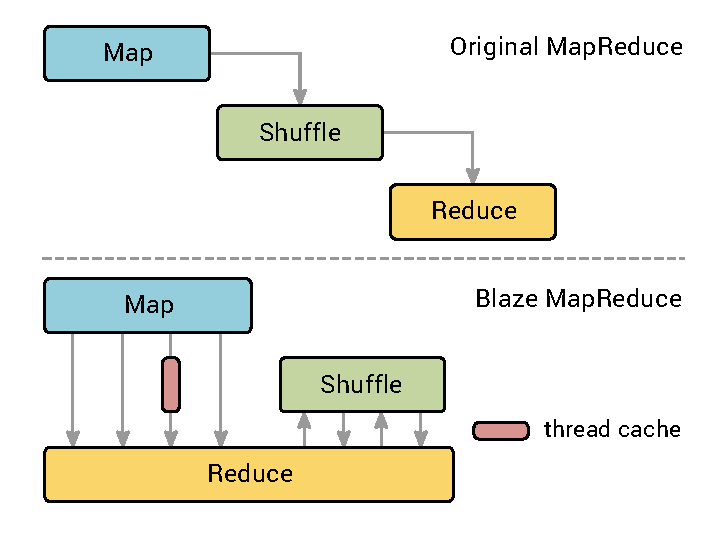
\includegraphics[width=\linewidth]{mrDiff0.eps}
  \end{center}
  \vspace{-0.2cm}
  \caption{Eager Reduction in Blaze MapReduce.
%   Blaze performs machine-local reduce right after the mapper function emits a key/value pair.
%   For popular keys, Blaze automatically reduce new values to a thread-local cache instead of the main copy on a machine.
%   The cross-machine shuffle operates on the locally reduced data and thus requires much less network communication.
%   During the shuffle operations, reduce operations also happen asynchronously to maximize the throughput.
  }
  \label{fig:mrdiff}
\end{figure}

In Blaze MapReduce, we perform machine-local reduce right after the mapper function emits a key/value pair.
For popular keys, Blaze automatically reduces new values to a thread-local cache instead of the machine-local copy.
The cross-machine shuffle operates on the locally reduced data which substantially reduces the network communication burden.
During the shuffle operations, reduce functions are also operating asynchronously to maximize the throughput.
Fig.~\ref{fig:mrdiff} illustrates the difference between the conventional MapReduce and Blaze MapReduce with eager reduction.

\subsubsection{Fast Serialization}
During the shuffle/reduce phase, we serialize the messages into a compact binary format before casting them across the network.

Our encoding scheme and algorithm are similar to Google's Protobuf~\cite{protobuf} but without prefixing each entry with field tags and wire types.
Although these two fields allow missing fields and support serializing the fields in arbitrary order, this additional flexibility is not needed in MapReduce.
On the other hand, these two fields can have a significant impact on both the performance and the serialized message size, especially when the content size of a field is small, which is common for MapReduce key/value pairs.
For example, when both the key and value are small integers, the serialized message size of each pair from Protocol Buffers will be 4 bytes while the message from Blaze fast serialization will be only 2 bytes, which is 50\% smaller than the one from Protocol Buffers.
Removing the fields tags and wire types does not cause ambiguity as long as we always serialize the fields in the same order, which is easy to achieve in MapReduce.
The smaller size in the serialized message means less network traffics, so that Blaze can scale better on large clusters when the cross-rack bandwidth becomes the bottleneck.

% \subsubsection{Hash-Based Shuffle}

% We use hash based shuffle instead of the original sort based shuffle.
% Hash based shuffle can send the messages to the corresponding worker in $O(1)$ time.

% Note that in the MapReduce results, the keys are no longer sorted.
% We provide a separate function, called \lstinline{top} for achieving similar capability in the distributed vector container.
% \lstinline{top} returns the top k elements in the distributed vector container in $O(n + k \log k)$ time, according to a custom compare function.
% When $k=n$, it will essentially perform a parallel merge sort.
% In section \ref{sec:nn}, we provide an example of the nearest 100 neighbors related to a given point from a huge set of other points, which uses the member function.

\subsubsection{Optimization for Small Key Range}

For small key range, we create a thread-local cache for each key at the beginning and set that as the reduce target during the local map/reduce phase.
After the local map/reduce phase finished, we perform parallel tree based reduce operations: first locally and then across multiple machines.
The resulting execution plan is essentially the same as hand-optimized parallel for loops with thread-local intermediate results.

\begin{table}
  \caption{Monte Carlo Pi Estimation Performance.
  We can see that Blaze MapReduce has almost the same speed as hand-optimized MPI+OpenMP parallel for loops while requires much fewer source lines of code (SLOC).}
  \label{tab:pi}
  \begin{tabular}{ccc}
    \toprule
    Samples & Blaze MapReduce & MPI+OpenMP\\
    \midrule
    $10^7$ & $0.14\pm 0.01$ s& $0.14\pm 0.01$ s \\
    $10^8$ & $1.44\pm 0.07$ s& $1.42\pm 0.09$ s \\
    $10^9$ & $14.2\pm 1.3$ s& $14.6\pm 1.7$ s \\
    \midrule
    SLOC & 8 & 24 \\
  \bottomrule
\end{tabular}
\end{table}

We benchmark the performance of Blaze MapReduce against hand-optimized parallel for-loop on the Monte Carlo Pi estimation task.
In this task, the mapper function first generates two random numbers $x$ and $y$ in the range $[0, 1]$, and then emits 1 to key 0 when $x^2 + y^2 < 1$.
Cases like this where we reduce big data to a small number of keys are commonly seen in data mining and are not efficient with the original MapReduce algorithm.
However, by using a thread-local copy as the default reduce target for each thread, Blaze MapReduce can achieve similar performance as hand-optimized code based on raw MPI and OpenMP.
Table~\ref{tab:pi} reports the result and Appendix~\ref{app:pi} lists our implementation.
The tests are performed on a local machine with Ubuntu 16.04, GCC 5.4 -O3, and an Intel i7-8550U processor.
